%!TEX root = main.tex
\section{Perspective Resolution in Crowdsourced Image Segmentation}
\subsection{Worker Clustering}
Our clustering-based approach is based on the intuition that workers with similar perspectives  will have segmentations that are closer to each other. We capture the similarity between a pair of workers by computing the Jaccard score between their segmentations and perform spectral clustering to separate workers into clusters. Figure \ref{cluster_example} illustrates how spectral clustering is capable of dividing the worker responses into clusters with meaningful semantic associations, reflecting the crowd's diversity of perspectives in completing same task.
    \begin{figure}[h!]
      \centering
      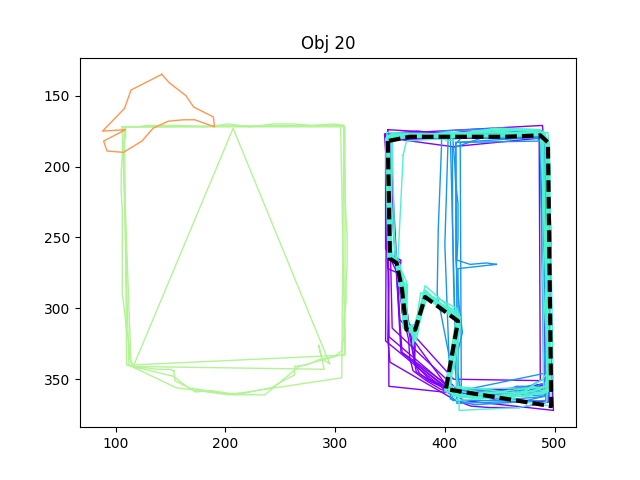
\includegraphics[width=\textwidth]{plots/20.png}
      \caption{Example image showing clustering performed on the same object from Figure \ref{error_examples}.}
      \label{cluster_example}
    \end{figure}
\par Clustering results can also be used as a preprocessing step to any of the quality evaluation algorithms by keeping only the segmentations that belong to the largest cluster, which is typically free of any semantic errors. As shown in Table~\ref{statsTable}, on average, clustering generally results in an increase the resulting algorithmic performance. Since the ground-truth supervised variants are already free of semantic ambiguity and errors, there is minimal improvement resulting from clustering. %In particular, we see a greater improvement with clustering preprocessing for algorithms that are not very robust in resolving semantic errors or ambiguity, such as for the \texttt{num pts} retrieval algorithm, than compared to the aggregation-based methods. 
\par Clustering offers an additional benefit of preserving worker's semantic intentions in the case where there are multiple instances of different errors. For example, in Figure \ref{cluster_example}, the mistakened clusters included semantic concepts ``monitor'' and ``turtle''. While these are considered \textit{bad} annotations for this particular task, this cluster of annotation can provide more data for another semantic segmentation task ``monitor''. A potential direction of future work includes adding an additional crowdsourcing task for semantic labelling of clusters (which is cheaper and more accurate than segmentation) to enable reuse of annotations across objects and lower the cost of data collection. 